\documentclass[UTF8]{ctexart}
\usepackage{graphicx}
\usepackage{amsmath}
\begin{document}

\title{半马尔可夫过程}
\author{庞海天}
\maketitle

半马尔可夫过程既可以认为是一个马尔科夫更新过程,又是马尔可夫过程的推广。马尔科夫更新过程关心推广的更新随机变量(例:它会记录整个过程中到达每个状态的数量),而半马尔可夫过程关心描述在某时刻的过程状态的随机变量。

离散事件马尔科夫过程中,我们假定每次转移之前在每个状态所停留的时间为单位时间。相似地,在连续时间马尔科夫过程中,我们假定每次停留之前在每个状态所停留的时间符合指数分布。半马尔可夫过程就是一个状态之间的转移像马尔科夫过程的随机过程。然而,在状态转移之前每个状态上所停留的时间是依赖于过程将要进入的状态的任意的随机变量。因此,在转移的瞬间上来看,半马尔可夫过程的表现和马尔科夫过程一样。

设状态空间S可数,$P=(p_{ij})$为S上的状态转移矩阵,即P满足$$\forall i,j \in S,p_{ij}\ge 0\quad \sum_{j\in S}p_{ij}=1$$

定义:设$X=\{X(t),t\ge 0\}$是状态空间S上的轨道右连续随机过程,称X为半马尔可夫过程,若满足:

$$X(t)=\sum_{n\ge 0}Y_nI(\tau_{n}\le t \le\tau_{n+1})$$

其中:

(1)$$\{Y_n,n\ge0\} \sim MC(\pi(0),\widetilde{P}),\quad \widetilde{P}=(\widetilde{p_{ij}}) $$

$$\forall i,j \in S, 0\le \widetilde{p_{ij}}\le 1;\sum_{j\in S}\widetilde{p_{ij}}=1$$

(2)$$\{\tau_n,n\ge1 \},\tau_0=0,\tau_n=\sum_{k=1}^n\theta_k$$

其中$\tau_n$为第n次跳的时刻,当给定$Y_0,...,Y_n=i,Y_{n+1}=j,...$时,$\theta_n$的分布函数为$F_{ij}(t)=P(\theta_n\le t|Y_0,...,Y_n=i,Y_{n+1}=j)\quad i,j\in S$

(3)若$\widetilde{p_{ii}}=1$,称i为吸收态。若$X(t)=i$,则

$$\forall h>0,X(t+h)=i$$

等价定义:设$X={X(t),t\ge 0}$是状态空间S上的轨道右连续随机过程,若对$\forall t,h\ge 0,i,j\in S$,在$X(t)=i $的条件下,$X(t+h)$和$\{X(s),0\le s < t\}$独立,如果$p_{ij}>0$,即状态i可以直接转移到状态j,若当前状态为i,选择了状态j之后,过程在状态i上停留的时间$\theta_{ij}$为一取值非负的随机变量,分布函数为$F(t),t \ge 0$,则称随机过程$X=\{X(t),t\ge 0\}$为半马尔可夫过程。其中,$\theta_{ij}$若取值非负实数,则X(t)为连续时间半马尔可夫过程,若取值为非负整数,则为离散时间半马尔可夫过程。

重要性质

1.$\forall w \in \Omega, X(t,w)$关于$t>0$为右连续左极限存在的上下随机跳跃的台阶形函数。

2.$\{\tau_n,n\ge1\},(\tau_0=0)$是跳跃时刻。

3.选择了$j$之后,随机过程在状态i上的停留时间为$\theta_{ij}$,$\theta_{ij}$是一个取值为正的随机变量。因此,状态i上停留时间$\theta_i$的概率分布为
$$P(\theta_{i} < m)=\sum_{j\in S} p_{ij}P(\theta_{ij} < m)$$
状态i上停留时间的期望为
$$E[\theta_{i}] = \sum_{j\in S} p_{ij}E[\theta_{ij}] \quad i=1,2,...,N$$

4.$Y_n$称为半马尔可夫过程$X_n$的嵌入马尔可夫链

5.如果嵌入马尔科夫链中的两个状态i,j是连通的,半马尔可夫过程中两状态也是连通的。且有$P[T_{ij}<\infty]\times P[T_{ji}<\infty]>0$

6.如果嵌入马尔科夫链中的状态i是常返态,半马尔可夫过程中该状态也是常返态。且有$P[T_{ii}<\infty]>0$

7.如果嵌入马尔科夫链中的状态i是瞬时态,半马尔可夫过程中该状态也是瞬时态。且有$P[T_{ii}<\infty]=0$


很多常用的随机过程都可以在此框架下进行表示。当停留时间$\theta_{ij}\equiv 1$,且仅在整数点取值时,该随机过程为一马尔科夫链。

当停留时间$\theta_{ij}$与$j$无关,且$\theta_{i}$是指数分布时,该过程为马尔可夫跳过程。

当停留时间$\theta_{ij}$与$i,j$无关时,半马尔可夫过程为马尔科夫更新过程。特别地,当$\theta$是指数分布时,该过程为泊松过程。

重生半马尔可夫过程

设$\{X(t),t\ge0\}$是一个半马尔可夫过程,n为非负整数,$\tau_n$表示第n次事件发生的时刻,$X^{(n)}(t)=X(\tau_n+t)-X(\tau_n)$为$\{X(t),t\ge 0\}$在$\tau_n$后的重生半马尔可夫过程,则$X^{(n)}(t)=X(\tau_n+t)-X(\tau_n)$与$X(\tau_n \bigwedge t)$相互独立。

\section{离散时间半马尔可夫过程}

\begin{figure}[htbp]
\centering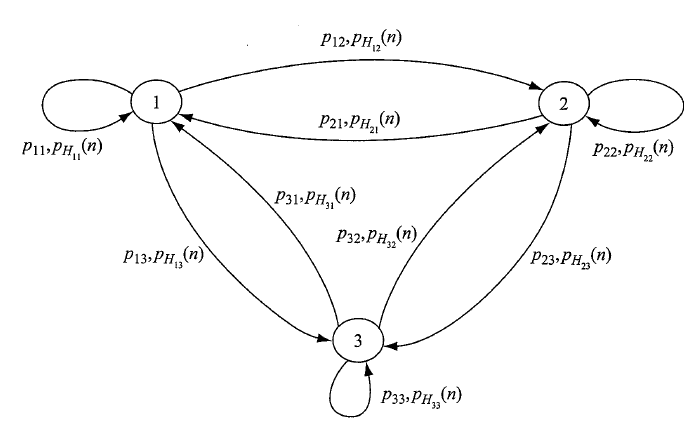
\includegraphics[width=3.5in]{f61}
\caption{离散时间半马尔可夫过程的状态转移图:它的嵌入马尔科夫链一共有三个状态。转移弧包含转移概率和条件停留时间的概率分布。}\label{fig:1}
\end{figure}

\subsection{转移概率}

用$\phi_{ij}(n)$来代表已知过程在$0$时刻处于状态$i$,$n$时刻位于状态$j$的概率,通常被称为状态$i$到状态$j$的转移概率函数。我们考虑$\phi_{ij}(n)$的两种取值情况:

a. 对于$i\ne j$,过程在时刻$m$转移到某个状态$k$,并在剩余的$n-m$时间内转移到状态$j$。这一事件的概率为:
$$\phi_{ij}(n)=\sum_{k \in S} p_{ik}\sum_{m=1}^n P(\theta_{ik}=m)\phi_{kj}(n-m) \quad i \ne j$$

b. 对于$i=j$,我们有一种额外的概率,即在感兴趣的时间段之内从未离开状态$i$。这一额外的概率为:
\begin{center}
$P[\theta_i>n]=1-P[\theta_i \le n]=1-F_{\theta_i}(n)$ 
\end{center}
由于从未离开状态$i$和离开$i$状态到达某个$k$状态是互斥的,所以有:
$$\phi_{ij}(n)=1-F_{\theta_i}(n)+\sum_{k \in S} p_{ik}\sum_{m=1}^n P(\theta_{ik}=m)\phi_{kj}(n-m) \quad i = j$$

如果定义
$$\delta_{ij}=
\begin{cases}
1 \quad i=j  \\
0 \quad i \ne j
\end{cases}$$
过程在时刻$m$转移到某个状态$k$,并在剩余的$n-m$时间内转移到状态$j$。这一事件的概率为:
$$
\begin{aligned}
\phi_{ij}(n)=\delta_{ij}[1-F_{\theta_i}(n)]+\sum_{k \in S} p_{ik}\sum_{m=1}^n P(\theta_{ik}=m)\phi_{kj}(n-m)
 \\=\delta_{ij}[1-F_{\theta_i}(n)]+\sum_{k\in S} p_{ik}P_{\theta_{ik}}(n)*\phi_{kj}(n) 
\end{aligned}
$$
其中$\phi_{ij}(0)=\delta_{ij}$,$*$为卷积符号。上述等式为半马尔可夫过程的后向$Chapman-Kolmogorov$等式。

用$P_\theta(n)$代表$P_{\theta_{ik}}(n)$组成的矩阵,$P$代表嵌入马尔科夫过程的状态转移矩阵。定义离散时间和矩阵$C(n)$为:
\begin{center}
$C(n)=P\bullet P_\theta(n)$
\end{center}

这就是说,$C(n)$的分量为$c_{ij}(n)=p_{ij}P_{\theta_{ij}}(n)$。因此,转移概率函数变成了:
\begin{center}
$\phi_{ij}(n)=\delta_{ij}[1-F_{\theta_i}(n)]+\sum c_{ik}(n)*\phi_{kj}(n) $
\end{center}
对上式两边同时取$z$变换得到:
\begin{center}
$\phi_{ij}(z)=\frac{\delta_{ij}[1-G_{\theta_i}(z)]}{1-z}+\sum c_{ik}(z)\phi_{kj}(z) $
\end{center}
其中$G_{\theta_i}(z)$是$P_{\theta_i}(n)$的$z$变换形式。用$D(z)$代表$N\times N$的对角方阵,其中第$i$个对角元素为${1-G_{\theta_i}(z)}/(1-z)$。于是,矩阵形式的等式就变成了:
\begin{center}
$\Phi(z)=D(z)+C(z)\Phi(z) $
\end{center}
如果定义

$$\phi_{ij}=\lim_{n\to \infty} \phi_{ij}(n) $$

可以得到:

$$\phi_{ij}=\frac{\pi_jE[\theta_j]}{\sum_{k\in S} \pi_kE[\theta_k]}$$

其中$\pi_j$是嵌入马尔科夫链的极限状态概率。可以看到等式右边是和$i$独立的,所以我们可以定义半马尔可夫过程的极限分布概率为:

$$\phi_j=\frac{\pi_jE[\theta_j]}{\sum_{k \in S} \pi_kE[\theta_k]}$$

极限状态概率分布也叫做占有率分布,因为 $\phi_j$可以显示过程长期的停留在状态$j$的比例。
$$\sum_{j\in S} \phi_j=1$$

\subsection{首达时间}
用$T_{ij}$表示第一次从状态$i$转移到状态$j$的时刻,即
\begin{center}
$T_{ij}=min\{n>0|X_n=j,X_0=i\}$
\end{center}
令$m_{ij}=E[T_{ij}]$,即$m_{ij}$是第一次从状态$i$转移到状态$j$的时刻平均值。我们可以如下迭代地得到$M_{ij}$,因为在状态$i$的平均停留时间是$E[\theta_i]$,如果已知一个过程从状态$i$开始,它在以概率$p_{ik}$转移到状态$k$之前停留的平均时间为$E[\theta_i]$,然后从状态$k$经过平均时间$m_{ij}$到达状态$j$。即
$$m_{ij}=E[\theta_i]+\sum_{k\in S,k\ne j} p_{ik}m_{kj} $$

当$j=i$时,即得到平均回转时间。特别地,因为嵌入马尔科夫链的极限状态概率分布存在,它们满足等式
$$\pi_i=\sum_{k\in S} \pi_kp_{ki}$$

$$
\begin{aligned}
\sum_{i \in S}\pi_im_{ij}=\sum_{i \in S}\pi_iE[\theta_i]+\sum_{i\in S}\pi_i\sum_{k\in S,k\ne j}p_{ik}m_{kj}  
\\= \sum_{i \in S}\pi_iE[\theta_i]+\sum_{k\in S,k\ne j}m_{kj}\sum_{i \in S}\pi_ip_{ik} 
\\ = \sum_{i \in S}\pi_iE[\theta_i]+\sum_{k \in S,k\ne j}m_{kj}\pi_k 
\\= \sum_{i \in S}\pi_iE[\theta_i]+\sum_{i\in S}\pi_im_{ij}-\pi_jm_{jj}
\end{aligned}
$$
等式左边右边消去后得到
$$m_{jj}=\frac{\sum_{i\in S}\pi_iE[\theta_i]}{\pi_j}\quad \forall j \in S$$

例1:

考虑一个人在3个地点(教学楼,宿舍,图书馆)之间进行移动,他的移动模型可以用一个离散时间的半马尔可夫过程来进行建模。分别设3个地点为$p_1=1,p_2=2,p_3=3$。转移矩阵为P,如图所示。在一个地点停留时间的分布取决于当前停留的地点与接下来将要到达的地点。设当前停留的地点为a(n),下一地点为a(n+1),停留时间的概率分布符合参数为$\lambda=\frac{p_{a(n+1)}}{p_{a(n)}}$的泊松分布。已知在$t=0$时刻,该人处于地点1。
\begin{center}
$P=
\left[
\begin{array}{c c c}
0 \quad 0.5 \quad 0.5\\
0.9 \quad  0 \quad  0.1\\
0.4 \quad  0.6 \quad  0
\end{array}
\right]$
\end{center}

a. 求该人首次离开地点1的时刻的概率分布函数和期望

b. 求该过程的占有率分布

解: a.设首次离开地点1的时刻为T,$T=n$的概率为:
$$\begin{aligned}
P(T=n)=p_{12}P(X=n,\lambda=2)+p_{13}P(X=n,\lambda=3)\\
=0.5*\frac{2^n}{n!}e^{-2}+0.5*\frac{3^n}{n!}e^{-3}
\end{aligned}$$
$$\begin{aligned}
E(\theta_i)=\sum_{n=1}^\infty n\times P(T=n)\\
=\sum_{n=1}^\infty np_{12}P(X=n,\lambda=2)+np_{13}P(X=n,\lambda=3)\\
=p_{12}\sum_{n=1}^\infty nP(X=n,\lambda=2)+p_{13}\sum_{n=1}^\infty nP(X=n,\lambda=3)\\
=p_{12}E(P.P(X,\lambda=2))+p_{13}E(P.P(X,\lambda=3))\\
=0.5*2+0.5*3\\
=2.5
\end{aligned}$$

b.由于状态空间有限,极限分布存在且等于平稳分布。$\pi=\pi P$,解得$\pi=(\frac{80}{229},\frac{94}{229},\frac{55}{229})$。由a.的结论可以类似地求出$E(\theta_2)=0.6,E(\theta_3)=\frac{8}{15}$

$$
\phi_1=\frac{\pi_1E(\theta_1)}{\sum_{k=1}^3 \pi_kE(\theta_k)} \approx 0.700
$$

同理可得
$$\begin{aligned}\phi_2\approx 0.197\\
\phi_3\approx 0.103\end{aligned}
$$
\section{连续时间半马尔科夫过程}
\begin{figure}[htbp]
\centering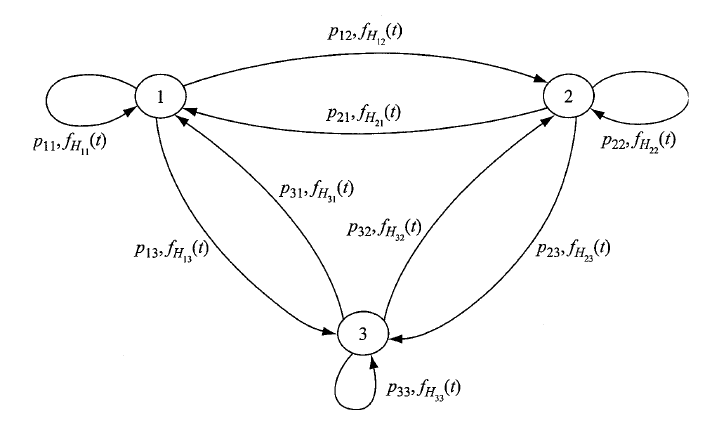
\includegraphics[width=3.5in]{f62}
\caption{连续时间半马尔可夫过程的状态转移图}\label{fig:2}
\end{figure}

\subsection{状态概率}

用$\phi_{ij}(t)$来代表已知过程在0时刻处于状态i,n时刻时位于状态j的概率,通常被称为状态i到状态j的转移概率函数。正如之前提到的,$\phi_{ij}(t)$被称为从状态i到状态j的转移概率函数。和离散时间的状况相同,我们考虑两种情况:

a. 对于$i\ne j$,过程在时刻u转移到某个状态k,并在剩余的t-u时间后到达状态j。这一事件的概率为:
$$\phi_{ij}(t)=\sum_{k\in S} p_{ik}\int_{u=0}^t f_{\theta_{ik}}(u)\phi_{kj}(t-u)du  \quad i \ne j $$

b.对于$i=j$,我们有一种额外的概率,即在感兴趣的时间段之内从未离开状态i。这一额外事件的概率为:
$$P[\theta_i>t]=1-P[\theta_i\le t]=1-F_{\theta_i}(t)  $$

由于从未离开状态i和离开i状态到达某个k状态是互斥的,所以有:
$$\phi_{ii}(t)=1-F_{\theta_i}(t)+\sum_{k\in S} p_{ik}\int_{u=0}^t f_{\theta_{ik}}(u)\phi_{ki}(t-u)du $$ 

于是,对于$i,j\in S$和$t \ge 0$,我们可以得到:
$$\phi_{ij}(t)=\delta_{ij}\{1-F_{\theta_i}(t)\}+\sum_{k\in S} p_{ik}\int_{u=0}^t f_{\theta_{ik}}(u)\phi_{kj}(t-u)du $$ 
其中$\phi_{ij}(0) = \delta_{ij}$。因为积分是一个卷积的形式,我们可以写成:
$$\begin{aligned}
\phi_{ij}(t)=\delta_{ij}\{1-F_{\theta_i}(t)\}+\sum_{k \in S} p_{ik}f_{\theta_{ik}}(t)*\phi_{kj}(t) \\
=\delta_{ij}\{1-F_{\theta_i}(t)\}+\sum_{k \in S} c_{ik}(t)*\phi_{kj}(t)
\end{aligned}
$$

与离散时间的情况相同,我们定义连续时间的核矩阵为
\begin{center}
$C(t)=[c_{ij}(t)]=P\bullet f_{H_t}=[p_{ij}f_{H_{ij}}(t)]$
\end{center}

我们定义$\phi_{ij}(s)$为$\phi_{ij}(t)$的s变换,$c_{ij}(s)$为$c_{ij}(t)$的s变换,并且注明$F_{\theta_i}(t)$的s变换为$M_{\theta_i}(s)/s$,其中$M_{\theta_i}(s)$是$f_{\theta_i}(t)$的s变换。因此,对上面等式两边进行s变换我们可以得到:
\begin{center}
$\begin{aligned}
\phi_{ij}(s)=\frac{\delta_{ij}}{s}\{1-M_{\theta_i}(s)\}+\sum c_{ik}\phi_{kj}(s) \\
=\frac{\delta_{ij}}{s}\{1-\sum p_{ik}M_{\theta_{ik}}(s)\}+\sum c_{ik}(s)\phi_{kj}(s)
\end{aligned}
$ 
\end{center}

最后,如果$D(s)$是$N\times N$的对角矩阵,且对角元素为${1-M_{\theta_i}(s)}/s$,矩阵形式的等式就变成了:

\begin{center}
$\Phi(s)=D(s)+C(s)\Phi(s)$
\end{center}

如果我们定义

\begin{center}
$$\phi_{ij}=\lim_{t \to \infty}\phi_{ij}(t)$$
\end{center}

有
\begin{center}
$$\phi_{ij}=\frac{\pi_jE[\theta_j]}{\sum_{k\in S} \pi_kE[\theta_k]}$$
\end{center}

其中$\pi_j$是嵌入马尔科夫链的极限概率分布。因为等式右边是与状态i独立的,我们能够得到半马尔科夫链的极限分布为:

\begin{center}
$\phi_{j}=\frac{\pi_jE[\theta_j]}{\sum_{k\in S} \pi_kE[\theta_k]}$
\end{center}

正如以前所说的,极限状态概率也叫做占有率分布,因为$\phi_j$能够反映长期以来过程处于状态j的时间的比例。



\subsection{首达时间}
用$T_{ij}$来表示首次从状态i转移到状态j的时刻。

\begin{center}
$T_{ij}=min\{t>0|X(t)=j,X(0)=i\}$
\end{center}

令$m_{ij}=E[T_{ij}]$,即$m_{ij}$是第一次从状态$i$转移到状态$j$的时刻平均值。在离散的情况下,我们有

\begin{center}
$m_{ij}=E[\theta_i]+\sum_{k\ne j} p_{ik}m_{kj}$
\end{center}

最后用同样的方法,我们可以获得平均回转时间为

\begin{center}
$m_{jj}=\frac{\sum_{i \in S} \pi_iE[\theta_i]}{\pi_j} \quad \forall j\in S$
\end{center}








\end{document}